\section{Approximating $E_n(\xi)$}\label{apxEn}
A significant barrier to analytically solving $\tilde R$ in the discrete maximum
principle statement is obtaining appropriate values for the
exponential integrals found therein.  An analysis is approached here that seeks
to compare an approximation of the exponential integral with an iterative
expansion method.

For computing purposes, an ideal approximation to the exponential integral
would deliver a simple set of terms that closely reflect the exponential
integral while proving much simpler to handle numerically.  One such expansion
is described online by the Wolfram group \cite{wolframEn}:

\begin{equation}
E_n(\xi)\approx\frac{e^{-\xi}}{\xi}\left(1-\sum_{i=0}^{n-1}
  \frac{\prod_{j=0}^i n+j}{\xi^{i+1}}\right)\label{En exp}
\end{equation}

Eq. \eqref{En exp} is an asymptotic expansion that should be truncated at a
number of terms equal to the order $n$ of the integral, hence the upper limit
in the sum.  To compare various numbers of terms kept, see Figure \ref{expint}
and \ref{expint_err}.  These graphs were generated of
the generic $E_3(\xi)$ approximation, which is of
central interest to us as this term appears in $\tilde R$. As can be readily
seen, the 2-term expansion coincides most quickly with the actual exponential
integral, which is expected given the $n-1$ term limit.  The benchmark for the
approximation is taken from a machine-precision code given in the Numerical
Recipes series, an iterative method for converging on exponential
integral values \cite{numRec}.
\begin{figure}[htb]
\centering
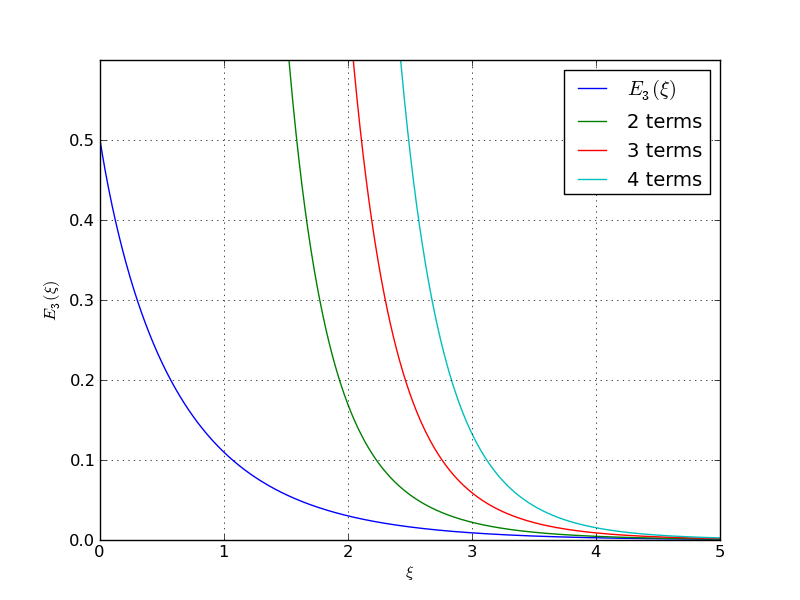
\includegraphics[width=0.7\linewidth]{expint_act}
\caption{Approximating $E_3(\xi)$}
\label{expint}
\end{figure}

\begin{figure}[htb]
\centering
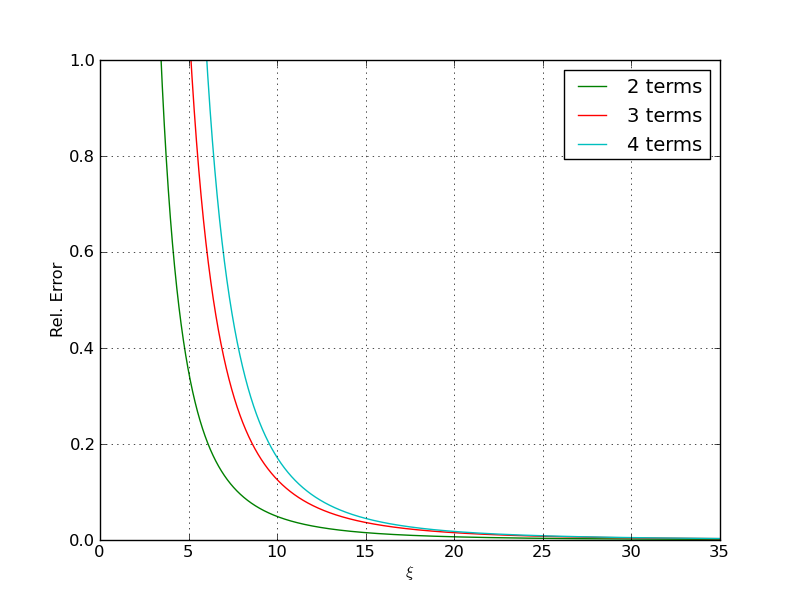
\includegraphics[width=0.7\linewidth]{expint_err}
\caption{Relative error in approximating $E_n(\xi)$}
\label{expint_err}
\end{figure}

The relative error between the two-term
approximation and the ``actual'' integral decreases exponentially, crossing 1\%
error just before $\xi=18$.  Imposing this 1\% error as a minimum, then, the
limits of this approximation can be derived.  Since the exponential
integral of interest is $E_3(\hat\Sigma\Delta_x)$, we have the following:
\[\hat\Sigma\Delta_x \geq 18, \]
\[\left(\sigma_0 + \frac{1}{c\Delta_t}\right)\Delta_x\geq 18. \]
Since $\sigma_0$ can vary significantly in form, we assume the user-defined
values $\Delta_x$ and $\Delta_t$ to be the limiting terms in this inequality. 
Thus, conservatively, we impose the inequality on only the right term of
$\hat\Sigma$:
\[(\sigma_0 + \frac{1}{c\Delta_t})\Delta_x>\frac{\Delta_x}{c\Delta_t}\geq 18.\]
Hence, a relative error of 1\% for this exponential integral can be obtained as
long as the following criterion is met:
\begin{align}
\frac{\Delta_x}{\Delta_t}&\geq \frac{18}{c} \nonumber \\
&\geq .060042 < 0.1
\end{align}
Thus, conservatively, a 1\% margin of error can only be retained by assuring the
ratio between $\Delta_x$ and $\Delta_t$ is greater than 0.1.

The significant limitations on user parameter choices discourages use of the
approximation without significant increase in efficiency.  In order to
determine the time benefit of the approximation \cite{wolframEn} against
the iterative expansion method \cite{numRec}, 500 runs to calculate $E_3(\xi)$
of each method were timed and set into a ratio for various values of argument
$\xi$.  The results are given in figure \ref{runtime}.
\begin{figure}[htb]
\centering
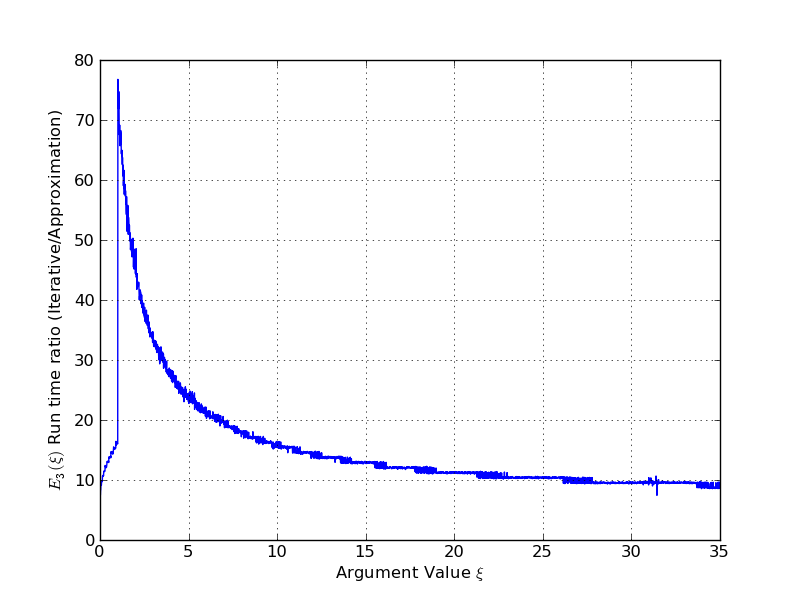
\includegraphics[width=0.7\linewidth]{exp_runtime}
\caption{Run time ratios for calculating $E_n(\xi)$: iteration vs approximation}
\label{runtime}
\end{figure}

The sudden increase at $\xi=1$ arises because of a switch in methodology. The
method for $\xi$ less than unity is a digamma series, while the 
method for greater $\xi$ is a continued fraction.  The two expansions in the
iterative method are as follows:
\[E_n(\xi<1)= \frac{(-\xi)^{n-1}}{(n-1)!}[-\ln \xi+\psi(n)]
    -\sum_{m=0,m\neq n-1}^\infty\frac{(-\xi)^m}{(m-n+1)m!},\]
\[E_n(\xi\geq1)=e^{-\xi}\left(\frac{1}{\xi+n-}\ \frac{1\cdot n}{\xi+n+2-}
    \ \frac{2(n+1)}{\xi+n+4-}...\right). \]

While the approximation approaches two orders of magnitude
faster than the expansion method near $\xi=1$, it is only an order of magnitude
faster when the
approximation is within 1\% error of the expansion method. 
Thus, the relatively minor gain in using the approximation is outweighed by its
restrictive useful range.  Hence, we intend to make use of the expansion
solution in computing terms of $E_3(\hat\Sigma x)$ instead of using the
asymptotic expansion.

